
\documentclass[12pt]{article}
\usepackage[letterpaper,textwidth=5.5in,right=0.6in,textheight=9in,left=0.6in,top=0.7in,bottom=0.7in]{geometry}

\usepackage{amsmath,amssymb}
\usepackage{graphicx}
\begin{document}
	\noindent Graph Theory HW 6\\
	Wang Xinshi, 661975305\\
	wangx47@rpi.edu\\
	
	\noindent 1.\text{\bf Proof:} Since $|V(G)| \geq 6$ and $G$ is $3$-connected, there must exists at least one vertex $v_p \in V(G)$(even if $v_p$ is in the subdivision of $K_5$) connecting to 3 vertices $v_a,v_b,v_c \in V(K_5)$; otherwise we could cut one or two edges between $v_p$ and $v_i \in V(K_5)$ to disconnect the graph so it is not 3-connected. Then Let us denote the vertex set $X = \{v_a,v_b,v_c\}$ and $Y = v_p \cup V(K_5) \setminus \{v_a,v_b,v_c\}$. Since every vertex in $K_5$ is connected to each other and $v_p$ is connected to all $v \in \{v_a,v_b,v_c\}$. Thus we have $\forall v_i \in X$,$\forall v_j \in Y$,$\exists (v_i,v_j)$ such that $(v_i,v_j) \in V(G)$. Therefore by definition we have a $K_{3,3}$.
	
	 	\hfill $\blacksquare$
	 	
	 \noindent 2.\text{\bf Proof:} In order to prove $\exists u,v\in V(G) : d(u) \leq 5, d(v) \leq 5$, we need to show (i).it cannot be the case that $\forall u \in V(G): d(u) > 5$. (ii). it cannot be the cast that there exists only one $v_p$ such that $\forall u \in V(G): d(u) > 5$ and $v_p \leq 5$.
	 
	 In order to show it cannot be the case that $\forall u \in V(G): d(u) > 5$, we use the necessary condition of a planar graph derived from Euler's formula: $m \leq 3n-6$, where $m = |E(G)|$ and $n = |V(G)|$. Thus we have $|E(G)| \leq 3|V(G)| - 6$. Let us assume $|V(G)| = n$. From the handshake theorem, we know
	 \begin{align*}
	 	\dfrac{\sum_{v \in V(G)}d(v)}{2} &\leq 3|V(G)|-6\\
	 	\dfrac{6n}{2} &\leq 3n-6  \text{\hspace{1in} Note: $\forall u \in V(G): d(u) > 5$}\\
	 	3n &\leq 3n-6\\
	 	0 &\leq -6
	 \end{align*}
 
 	Therefore we have arrived a contradiction. Thus it cannot be the case that  $\forall u \in V(G): d(u) > 5$.
 	
 	In order to show it cannot be the cast that there exists only one $v_p$ such that $\forall u \in V(G): d(u) > 5$ and $v_p \leq 5$,  we use the necessary condition of a planar graph derived from Euler's formula with the handshake theorem. Assume $\exists v \in V(G)$ s.t. $d(v) = k <= 5$. Thus we have 
 	\begin{align*}
 		\dfrac{\sum_{v \in V(G)}d(v)}{2} &\leq 3|V(G)|-6\\
 		\dfrac{6(n-1)+k}{2} &\leq 3n-6\\  
 		3n - 3 + k &\leq 3n-6\\
 		k &\leq -3
 	\end{align*}
	 
	Therefore we have arrived a contradiction. Thus it cannot be the case that there exists only one $v_p$ such that $\forall u \in V(G): d(u) > 5$ and $v_p \leq 5$. 
	
	Since we have eliminated the case where no vertex in G such that degree is less than or equal to 5 and there exists only one vertex in G such that degree is less than or equal to 5, there must have at least 2 vertices in G such that degree is less than or equal to 5.
	
		\hfill $\blacksquare$
		
	\newpage
		
	\noindent 3. \text{\bf Definition:} Given graph G, we can construct a graph G' with $V(G') = V(G) \cup \{v_{new}\}$. We then connect $v_{new}$ with all vertex $v \in V(G)$.
	
	\text{\bf Proof:} In order to show $G$ is outer-planar $\iff$ $G$ does not contain a $K_4$ or $K_{2,3}$ subdivision, we show (i). G is outer-planar $\iff$ G' is planar. (ii). $K_4 \subseteq G \iff K_5 \subseteq G'$. (iii).  $K_{2,3} \subseteq G \iff k_{3,3} \subseteq G'$. If the 3 claims above are true, it is obvious we can show the if direction by
	$$K_{2,3} \nsubseteq G \land K_4 \nsubseteq G \implies K_{3,3} \nsubseteq G' \land K_5 \nsubseteq G' \implies \text{G' is planar} \implies \text{G is outer-planar} \text{  (1)}$$   
	
	Similarly, we can prove the only if direction by
	$$\text{G is outer-planar} \implies \text{G' is planar} \implies K_{5} \nsubseteq G \land K_{3,3} \nsubseteq G \implies K_{4} \nsubseteq G' \land K_{3,3} \nsubseteq G' \text{  (2)}$$ 
	
	\text{\bf Claim 1:} G is outer-planar $\iff$ G' is planar.
	
	If G is outer-planar, we can  we can draw $v_{new}$ and its adjacent edges into the outer face,
	obtaining a planar drawing of G'. Since $G$ is outer-planar, thus no edges would cross after adding $v_{new}$. Thus $G'$ is planar. If $G'$ is planar, then we are left with only the contour of $G$ by the definition of our construction of $G'$. Thus $G$ is outer-planar.
	
	\text{\bf Claim 2:}  $K_4 \subseteq G \iff K_5 \subseteq G'$
	
	If $K_4 \subseteq G$, then by the definition of our construction $\exists H \subseteq G'$ with $V(H) = V(K_4) \cup \{v_{new}\}$ and edges connecting every pair of vertices in $V(H)$. Thus by definition we have a $K_5$.
	 
	If $K_5 \subseteq G'$, then removing $v_{new}$ from $G'$ decrease the degree of all vertices by one. Thus $\exists H \subseteq G$ with $V(H) = V(K_5) \setminus \{v_{new}\}$ and edges connecting every pair of vertices in $V(H)$. Thus by definition we have a $K_4$. Thus we have proved the claim is valid.
	
	\text{\bf Claim 3:}  $K_{2,3} \subseteq G \iff k_{3,3} \subseteq G'$
	
	If $K_{2,3} \subseteq G$, we can let $X = \{v_1,v_2\} \subset H$ denote the independent set with 2 vertices and $Y = \{v_3,v_4,v_5\} \subset H$ denote the independent set with 3 vertices. Since $\forall v \in G$, $\exists (u_{new},v) \in E(G')$ and $\forall u_1 \in X$, $\forall v_1 \in Y$, $\exists (u_1,v_1) \in E(G')$, we can form an independent set $X' = \{v_1,v_2,v_3\}$ so $\forall u \in X'$, $\forall v \in Y$, $\exists (u,v) \in E(G')$. 
	
	If $K_{3,3} \subseteq G'$, we know $\exists X \subset G = \{v_1,v_2,v_{new}\} \land \exists Y \subset G = \{v_4,v_5,v_6\}$ so $\forall u \in X$, $\forall v \in Y$, $\exists (u,v) \in E(G')$. After removing $v_{new}$ from $X$, we get $X' = \{v_1,v_2\}$. We know $\forall u \in Y$, $\forall v \in X'$, $\exists (u,v) \in G$ and vice versa by definition of our construction and $K_{3,3}$. Thus $\exists K_{2,3} \subseteq G$. 
	
	Since we have proved these three claims are true, following the path (1) and (2) we showed above gives us the conclusion that $G$ is outer-planar $\iff$ $G$ does not contain a $K_4$ or $K_{2,3}$ subdivision. 
	
		\hfill $\blacksquare$
		
	\noindent 4. \text{\bf Proof:} We prove the 2 color theorem using induction on the number of lines $n$.
	
	Base Case: $P(1)$. This is trivial to see. Since a line divides a plane into at most 2 maps, we can obviously color the 2 maps with 2 colors.
	
	Inductive Step: Assume $P(k<n)$ =  "a planed divided by $k$ lines are 2 colorable"  is valid, show $P(n)$ is valid.
	
	Since adding a line to a plane will only divide blocks with 1 color to 2 separate blocks, let us denote the set of blocks being divided after adding new line l as $\{B_1,B_2,..., B_n\}$. We pick an arbitrary block $B_i \in \{B_1,B_2,..., B_n\}$ and show with the addition of the new block we can still color the map with 2 colors. 
	
	Let us denote the left plane after adding $l$ as $H_l$ and the right plane as $H_r$. We then swap the color of $H_l$ and leave the coloring for $H_r$ unchanged. Since we are dividing block $B_i$ into 2 parts and $B_i$ has 1 color before adding $l$, reversing the color on one side makes sure the 2 parts for $B_i$ has opposite color. Since our choice of $B_i$ is arbitrary, we can do the same thing for all blocks. Thus we can still color the map after adding $l$. Therefore we have proved any such map is 2-colorable.
	
	\hfill $\blacksquare$
	
	\noindent 5. In order to prove for a maximum planar graph $G$, $\forall v \in V(G) : d(v) = \text{even} \iff \chi(G) \leq 3$ holds, we need to show (i). $\forall v \in V(G) : d(v) = \text{even} \implies \chi(G) \leq 3$. (ii). $ \chi(G) \leq 3 \implies \forall v \in V(G) : d(v) = \text{even}$.\\
	
	Let us first prove $(i)$ is valid. If $\forall v \in V(G) : d(v) = \text{even}$, we know $G$ is a even graph, which means G is Eulerian. We then prove this using induction on the number of faces in $G$. Let P(n) denote the statement maximal planar even graph $G$ with n faces has $\chi(G) = 3$. 
	
	Base Case: $P(1)$ is valid since we can cover one triangle(result from maximal planar) in 3 colors.
	
	Inductive hypothesis: Assume $P(1 \leq k < n) = $ maximal planar even graph $G$ with n faces has $\chi(G) = 3$ is still valid. Prove $P(n)$ is valid.
	
	Let e=xy be an edge on the exterior face of G. There must be an internal face containing xy. Let z be the common neighbor of x and y forming the internal face xyz. Consider 3 exhaustive cases:
	
	1. G is the triangle xyz. This is trivial to see.
	
	2. z is on the exterior boundary of G. In this case one among x and y - say x must have degree 2, and xz must be an edge on the exterior face of G. Consequently, $G \setminus \{x\}$ must be a 2-connected near triangulation with fewer internal faces, and must thereby admit an inductive 3-coloring. Put x back and a free color will be available to color x.
	
	3. z is an internal vertex. As G is a near triangulation, there must be a wheel, say W(z) in G with z at the center and an even number of vertices around z. As there are three vertex disjoint paths in W(z) between x and y, we can see that $G \setminus e$ is a 2-connected near triangulation with fewer faces. Consequently,$G \setminus e$ must be 3-colorable (by induction hypothesis). The path from x to y in $G \setminus e$ along the rim of W(z) contains even number of vertices. Further, the vertices in the path must be 2-colored (the color assigned to z cannot be assigned to them). Consequently, x and y must be colored differently in $G \setminus e$. Put the edge e back and we can color the graph with 3 colors.

	Let us next prove $(ii)$ is valid. Suppose $\exists v \in V(G)$ with odd degree. Now look at $N(v)$. Since $G$ is maximal planar, we know $N(v) \geq 3$, and they must be connected in a wheel graph with v at the center. The chromatic number of a wheel graph with an odd length outer cycle is 4. Thus we have a contradiction. Thus $\forall v \in V(G) : d(v) = \text{even}$.
		\hfill $\blacksquare$
		
	\noindent 6. \\
	
	(a). Since $b_1,b_2$, and $b_3$ are planar, we can make the 3 blocks on the same line. Since there must exists some vertex that is not contained in any face in $b_1$ and there must exists some vertex that is not contained in any face in $b_3$, we can connect those 2 vertices to get $G'$.
	
	\hfill $\blacksquare$
	
	(b). Since G' is a minimal non-planar graph, removing any any from G' makes G' a planar graph. Therefore $G = G' - e$ is a planar graph.
	
	\hfill $\blacksquare$
	\newpage
	(c). The graph has exactly $|V(G)| = 6$ and $|E(G)| = 11$. It is not planar because $K_5$ is clearly a subgraph of G.
			\begin{figure}[h]
				\begin{center}
						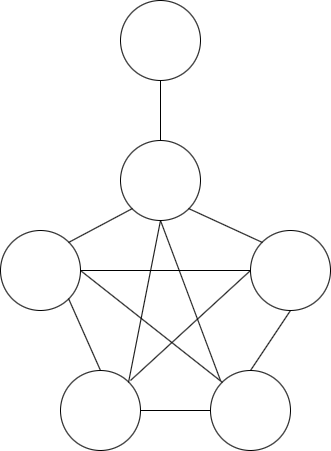
\includegraphics[scale = 0.3]{"C:/Users/Micha/OneDrive - Rensselaer Polytechnic Institute/Graph Theory/pictures/hw6-1.png"}\\
				\end{center}
		
		\end{figure}
	
	\hfill $\blacksquare$
	 
	
	(d). In order to prove $G'$ is planar $\implies$ $G=G' \cdot e$, where $e \in E(G')$, is planar, we can prove the contrapositve statement $G = G' \cdot e$ has kuratowski subgraph $\implies$ $G'$ has kuratowski subgraph.
	
	Let z be the vertex of G e obtained by contracting e = xy. If z is not in H, then H itself is a Kuratowski subgraph of G. If z $\in$ V (H) but z is not a branch vertex of H, then we obtain a Kuratowski subgraph of G from H by replacing z with x or y or with the edge xy.
	
	Similarly, if z is a branch vertex in H and at most one edge incident to z in H is incident to x in G, then expanding z into xy lengthens that path, and y is the corresponding branch vertex for a Kuratowski subgraph in G.
	
	In the remaining case (shown below), H is a subdivision of $K_5$ and z is a branch vertex, and the four edges incident to z in H consist of two incident to x and two incident to y in G. In this case, let $u_1,u_2$ be the branch vertices of H that are at the other ends of the paths leaving z on edges incident to x in G, and let $v_1$ , $v_2$ be the branch vertices of H that are at the other ends of the paths leaving z on edges incident to y in G. By deleting the $u_1$, $u_2$ -path and $v_1$, $v_2$-path
	from H, we obtain a subdivision of $K_{3,3}$ in G, in which y, $u_1$, $u_2$ are the branch vertices for one partite set and x, $v_1$ , $v_2$ are the branch vertices of the other.
		\begin{figure}[h]
		\begin{center}
			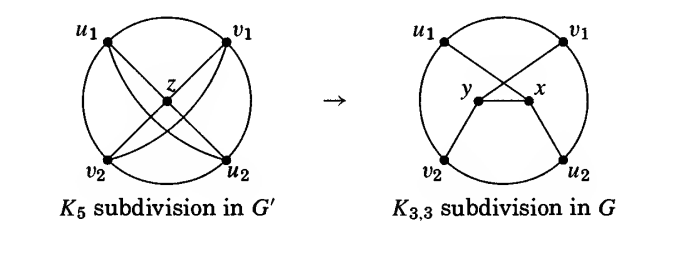
\includegraphics[scale = 0.6]{"C:/Users/Micha/OneDrive - Rensselaer Polytechnic Institute/Graph Theory/pictures/hw6-3.png"}\\
				\hfill $\blacksquare$\\
		\end{center}
		
	\end{figure}

	\newpage
	(e). As we can see, The graph contains a $K_{3,3}$ subdivison and it has $\chi(G) = 3$. Thus it is not planar.	
	\begin{figure}[h]
		\begin{center}
			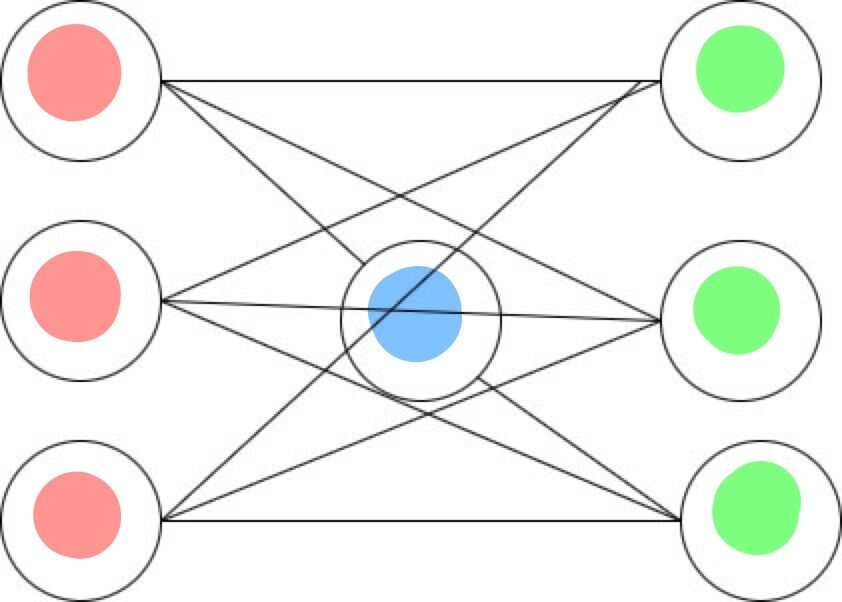
\includegraphics[scale = 0.2]{"C:/Users/Micha/OneDrive - Rensselaer Polytechnic Institute/Graph Theory/pictures/hw6-2.jpg"}\\
		\end{center}
		
	\end{figure}

	\hfill $\blacksquare$
\end{document}